
En esta segunda actividad pr\'actica nos centraremos en la correcci\'on radiom\'etrica
de imagenes satelitales. Son nuestros objetivos:

\begin{itemize}
    \item Abrir una imagen satelital desde el metadato.
    \item Convertir los valores de la imagen a reflectancia tope de la
        atm\'osfera.
    \item Corregir la imagen satelital utilizando los m\'etodos de \emph{dos} y
        \emph{cost}
    \item Corregir la imagen satelital utilizando el \emph{6S} en su versi\'on web.
\end{itemize}

\subsection{C\'alculo de reflectancia a tope de la atmosfera}

Para poder convertir una imagen a reflectancia a tope de la atm\'osfera vamos a
necesitar no solo la imagen sino tambi\'en la informaci\'on adicional que hallaremos
en su metadato.

Para abrir una imagen satelital desde el metadato utilizaremos las funciones
disponibles en la libreria \texttt{RStoolbox}. Esta incluye diversas herramientas
para trabajar con im\'agenes satelitales.

\begin{exa}
    Abramos  la imagen Landsat 7
    del año 2000 desde el metadato y la mostraremos en combinacion color real.
    Adem\'as analicemos sus propiedades.
    \begin{lstlisting}
    meta.2000 <- readMeta("raster_data/LE72240782000188EDC00/LE72240782000188EDC00_MTL.txt")
    \end{lstlisting}
    Podemos mostrar las distintas variables incluidas en el objeto usando el
    signo \$ y su nombre. Por ejemplo \verb|meta.2000$SOLAR_PARAMETERS|
    da como resultado
    \begin{Verbatim}[fontsize=\small]
     azimuth elevation  distance
    37.38251  31.14409   1.01670
    \end{Verbatim}
    Usando el metadato podemos cargar la imagen completa con el comando
    \texttt{stackMeta}. Ademas eliminaremos en este caso las bandas 6 y 7 por
    ser termicas.
    \begin{lstlisting}
    dn.2000 <- stackMeta(meta.2000)
    dn.2000 <- dn.2000[[-6:-7,]]
    dn.2000
    \end{lstlisting}
    obtenemos como resultado un objeto \emph{raster stack} como el que sigue
    \begin{Verbatim}[fontsize=\small]
    class       : RasterStack
    dimensions  : 2412, 1834, 4423608, 6  (nrow, ncol, ncell, nlayers)
    resolution  : 30.00402, 30.00265  (x, y)
    extent      : 731118.6, 786146, 7101531, 7173897  (xmin, xmax, ymin, ymax)
    coord. ref. : +proj=utm +zone=21 +south +datum=WGS84 +units=m +no_defs
                  +ellps=WGS84 +towgs84=0,0,0
    names       : B1_dn, B2_dn, B3_dn, B4_dn, B5_dn, B7_dn
    min values  :     0,     0,     0,     0,     0,     0
    max values  :   255,   255,   255,   255,   255,   255
    \end{Verbatim}
    Mostramos la imagen en cobinaci\'on de color real con \texttt{plotRGB(dn.2000, r=3, g=2, b=1, stretch="lin")}
    obteniendo la figura \ref{fig:dn-l7-rgb}.
     \begin{figure}[h!]
     \begin{center}
         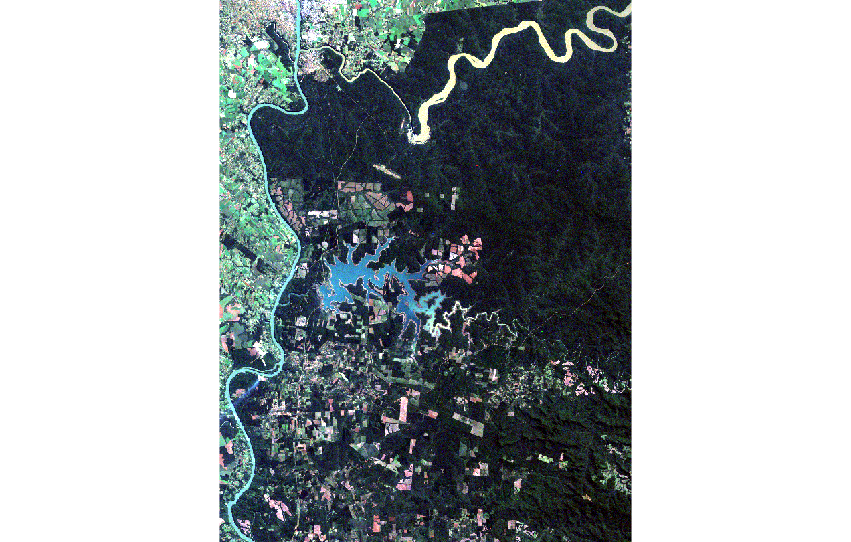
\includegraphics[scale=0.6]{dn-l7-rgb}
     \end{center}
     \caption{Imagen en combinaci\'on de bandas color real de la zona de interes.}
     \label{fig:dn-l7-rgb}
     \end{figure}
\end{exa}

De esta forma tenemos el archivo cargado en n\'umero digital con todos sus metadatos
para convertirlo a reflectancia y realizar distintas correcciones.

Para pasar nuestra imagen a reflectancia a tope
de la atmosfera tenemos dos maneras de hacerlo. Podemos hacerlo a mano
utilizando las herramientas algebraicas de R o podemos hacerlo con la funcion
especifica de \texttt{RStoolbox}.

\begin{exa}
    Calculo de reflectancia a tope de la atm\'osfera
    utilizando el metadato paso por paso

    \begin{lstlisting}
    dn2ref.2000 <- meta.2000$CALREF[1:6,]
    elev.2000 <- pi*meta.2000$SOLAR_PARAMETERS['elevation']/180
    \end{lstlisting}
    extraemos primero del metadatos los par\'ametros de calibraci\'on en
    reflectancia y el \'angulo de elevaci\'on solar. Convertimos luego la imagen
    a reflectancia y la dividimos por el seno del \'angulo solar.
    Luego cambiamos los nombres de las bandas

    \begin{lstlisting}
    toam.2000 <- (dn.2000*dn2ref.2000$gain+dn2ref.2000$offset)/sin(elev.2000)
    names(toam.2000) <- c("blue","green","red","nir","swir1","swir2")
    \end{lstlisting}

    Otra forma de realizar este proceso es utilizando la funci\'on
    \texttt{radCor}. En este caso debemos dar la imagen en DN, el metadato y
    cual es la cantidad que queremos calcular.

    \begin{lstlisting}
    toa.2000 <- radCor(dn.2000, metaData = meta.2000, method = "apref")
    \end{lstlisting}

    Podemos comparar los resultados de ambos metodos inspeccionando los objetos
    \texttt{toam.2000} y \texttt{toa.2000}.
    \begin{Verbatim}[fontsize=\small]
    class       : RasterBrick
    dimensions  : 2412, 1834, 4423608, 6  (nrow, ncol, ncell, nlayers)
    resolution  : 30.00402, 30.00265  (x, y)
    extent      : 731118.6, 786146, 7101531, 7173897  (xmin, xmax, ymin, ymax)
    coord. ref. : +proj=utm +zone=21 +south +datum=WGS84 +units=m +no_defs
                  +ellps=WGS84 +towgs84=0,0,0
    data source : in memory
    names       :        blue,       green,         red,         nir,    swir1,       ...
    min values  : -0.01976113, -0.02181530, -0.02029439,  0.01934678,    -0.02781926, ...
    max values  :   0.6106812,   0.5609009,   0.6079443,   0.8696885,    0.8640919,   ...
    \end{Verbatim}

    y

    \begin{Verbatim}[fontsize=\small]
    class       : RasterStack
    dimensions  : 2412, 1834, 4423608, 6  (nrow, ncol, ncell, nlayers)
    resolution  : 30.00402, 30.00265  (x, y)
    extent      : 731118.6, 786146, 7101531, 7173897  (xmin, xmax, ymin, ymax)
    coord. ref. : +proj=utm +zone=21 +south +datum=WGS84 +units=m +no_defs
                  +ellps=WGS84 +towgs84=0,0,0
    names       :     B1_tre,     B2_tre,     B3_tre,     B4_tre,     B5_tre, ...
    min values  : 0.00000000, 0.00000000, 0.00000000, 0.01934678, 0.00000000, ...
    max values  :  0.6106812,  0.5609009,  0.6079443,  0.8696885,  0.8640919, ...
    \end{Verbatim}

    \end{exa}

\begin{act}
    Inspeccione la reflectancia a tope de la atmosfera para todas las bandas.
    Para esto realice los histogramas, graficos de dispersi\'on, calcule la media,
    el desvio standar y cualquier otra medida estad\'istica que le guste.
\end{act}
\subsection{C\'alculo de reflectancia corregida atmosfericamente por m\'etodos
            estad\'isticos}

La funci\'on \texttt{radCor} dispone de un par\'ametro para hacer distintos
tipos de correcciones atmosf\'ericas. Ya vimos \emph{apref} que nos permiti\'o
calcular la reflectancia a tope de la atm\'osfera. Veamos como aplicar el m\'etodo
de substracci\'on de cuerpo obscuro.

\begin{exa}
    Apliquemos el metodo de \emph{simple dos} para corregir la imagen. En este caso
    solamente restaremos el m\'inimo en cada banda a la imagen para las bandas
    donde existe haze, es decir en la zona del visible y del infrarrojo cercano.

    Estimamos el haze primero y corregimos la imagen luego haciendo
    \begin{lstlisting}
    haze.2000 <- estimateHaze(dn.2000,darkProp = 0.01, hazeBands = 1:4, plot=TRUE)
    sdos.2000 <- radCor(dn.2000, metaData = meta.2000,
                 hazeValues = haze.2000,
                 hazeBands = c("B1_dn","B2_dn","B3_dn","B4_dn"),
                 method="sdos")
    \end{lstlisting}
    en este caso los valores de haze estimados son
    \begin{Verbatim}[fontsize=\small]
    B1_dn B2_dn B3_dn B4_dn
       41    27    20    15
    \end{Verbatim}
    Para hacer un an\'alisis de lo que pasa en la situacion, vamos a graficar los
    histogramas de cada banda para la imagen en reflectancia TOA y corregida por
    el m\'etodo \emph{simple dos}. Para esto usaremos el paquete \texttt{rasterVis}
    \begin{lstlisting}
    B1 <- densityplot(~B1_tre+B1_sre, data=toa.boa, xlab="Reflectancia",
                      ylab="", main="Banda azul", plot.points=FALSE, xlim=c(0,0.3),
                      key=simpleKey(text=c("Tope de la atmosfera",
                                           "Correccion Simple DOS"),
                                           lines=TRUE, points=FALSE))
    B2 <- densityplot(~B2_tre+B2_sre, data=toa.boa, xlab="Reflectancia",
                      ylab="", main="Banda verde", plot.points=FALSE, xlim=c(0,0.3),
                      key=simpleKey(text=c("Tope de la atmosfera",
                                           "Correccion Simple DOS"),
                                           lines=TRUE, points=FALSE))
    B3 <- densityplot(~B3_tre+B3_sre, data=toa.boa, xlab="Reflectancia",
                      ylab="", main="Banda roja", plot.points=FALSE, xlim=c(0,0.3),
                      key=simpleKey(text=c("Tope de la atmosfera",
                                           "Correccion Simple DOS"),
                                           lines=TRUE, points=FALSE))
    B4 <- densityplot(~B4_tre+B4_sre, data=toa.boa, xlab="Reflectancia",
                      ylab="", main="Banda nir", plot.points=FALSE, xlim=c(0,0.3),
                      key=simpleKey(text=c("Tope de la atmosfera",
                                           "Correccion Simple DOS"),
                                           lines=TRUE, points=FALSE))
     print(B1,split = c(1, 1, 2, 2),more=TRUE)
     print(B2,split = c(2, 1, 2, 2),more=TRUE)
     print(B3,split = c(1, 2, 2, 2),more=TRUE)
     print(B4,split = c(2, 2, 2, 2),more=FALSE)
    \end{lstlisting}
    En este caso las primeras 4 funciones crean los histogramas para cada banda
    corregida mientras que las \'ultimas 4 lineas los imprimen en una grilla como
    se ve en la figura \ref{fig:simpledos}.
    \begin{figure}[h!]
    \begin{center}
        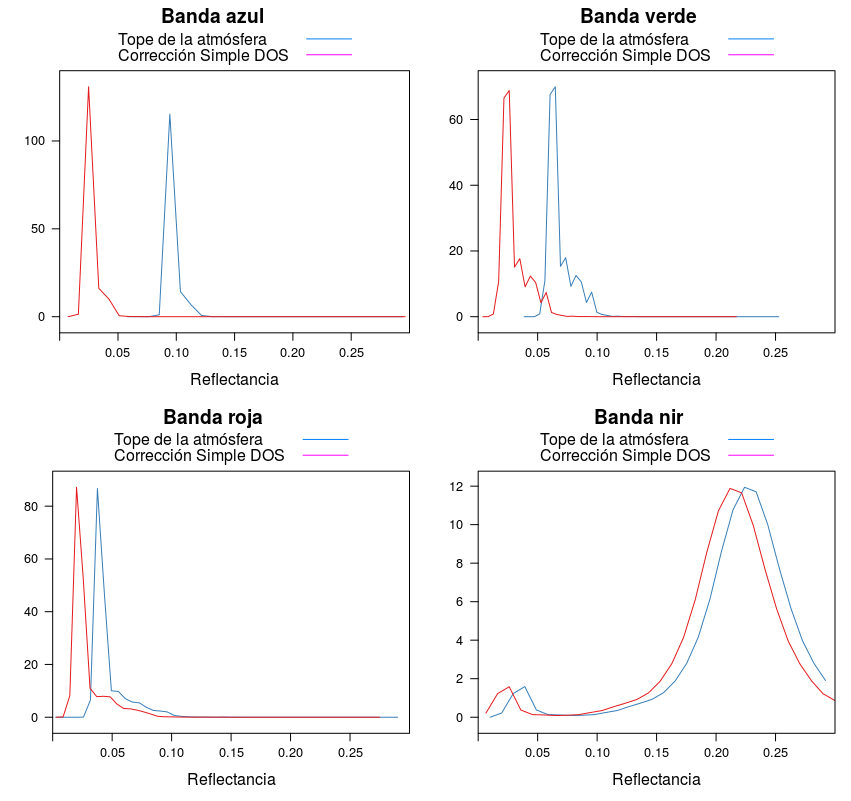
\includegraphics[scale=0.4]{simpledos.png}
    \end{center}
    \caption{Graficos de densidad para las distintas bandas donde se
        muestra el nivel de correcci\'on en cada una.}
    \label{fig:simpledos}
    \end{figure}
Notamos en este caso que la correccion se vuelve menos importante a medida
que crece la longitud de onda. adem\'as, la corecci\'on solo cambia la
posici\'on de la distribuci\'on y no su forma.

\end{exa}
\begin{act}
    Analice los valores de haze obtenidos por la funcion stimate haze y grafiquelos
    como funci\'on de la longitud de onda en escala logaritmica. ¿Que observa?
\end{act}

\begin{act}
    Utilice el m\'etodo \emph{costz} para corregir la imagen a reflectancia a tope
    de la superficie. Puede ayudarse con el comando \texttt{?radCor}
\end{act}

\begin{act}
    Guarde el archivos raster generado por cada uno de los m\'etodos de
    correcci\'on. Abralos en QGIS y comparelos visualmente. Obtenga firmas
    espectrales con los distintos m\'etodos de correccion.
\end{act}


\subsection{6S}
\label{sub:corr:6S}

Veamos ahora como operar con el 6S para obtener una estimaci\'on de los par\'ametros
atmosf\'ericos. Para esto utilizaremos la versi\'on web del 6S que se encuentra
disponible en \url{http://6s.ltdri.org/pages/run6SV.html}.

Para utilizarla ingresaremos a la pagina y haremos click en el boton
\menu{Submit query}. Iremos luego configurando paso a paso nuestro modelo de la
atm\'osfera haciendo siempre luego click en el bot\'on \menu{submit query} para
pasar al paso siguiente.

Los parametros para nuestro modelo son

\begin{enumerate}
    \item Geometrical conditions
        \begin{itemize}
            \item TM (Landsat)
            \item Month: 4, Day:13, GTM decimal hour: 13.60, Longitude:
                -63.8606, Latitude: -24.9937.
        \end{itemize}
    \item Atmospheric Model
        \begin{itemize}
            \item Select Atmospheric Profile: Mid latitude summer
            \item Select aerosol model: Continental Model
            \item Visibility: 60
        \end{itemize}
    \item Target \& sensor altitude
        \begin{itemize}
            \item Select targe altitude: sea level
            \item Select sensor altitude: satellite level
        \end{itemize}
    \item Spectral conditions
        \begin{itemize}
            \item Select spectral conditions: choose band
            \item Select band: 1st band of tm (landat 5)
        \end{itemize}
    \item Ground reflectance
        \begin{itemize}
            \item Ground reflectance type: homogeneous surface
            \item Directional effect: no directional effect
            \item Specify surface reflectance: input constant value of ro
            \item input constant value for ro: 0
        \end{itemize}
    \item Signal
        \begin{itemize}
            \item Atmospheric correction mode: no atmospheric correction
        \end{itemize}
\end{enumerate}

Todos estos valores los encontramos en el metadato de la imagen.

En \menu{7.Results} podemos ver el resultado haciendo click en \emph{Output
file}. Del mismo debemos extraer los valores de
 \begin{itemize}
     \item \texttt{global gas. trans. - total}
     \item \texttt{total sca. trans. - total}
     \item \texttt{spherical albedo - total}
     \item \texttt{reflectance I - total}
 \end{itemize}

Una vez ejecutado el proceso puede usarse el siguiente c\'odigo para corregir
todas las bandas utilizando R.

\begin{lstlisting}
    a <- c(0.98,0.90,...) # Global gas transmitance
    b <- c(0.81,0.90,...) # Total scatering transmitance
    g <- c(0.15,0.10,...) # Spherical albedo
    r <- c(0.08,0.05,...) # Reflectance I
    sss.2000 <- (toa.2000/(a*b)-r/b)/(1+g*(toa.2000/(a*b)-r/b))
\end{lstlisting}


\begin{act}
    Realice una extracci\'on de firmas espectrales para distintass coberturass de
    cada uno de los archivos raster obtenidos y grafiquelos juntas.
    Comparela con la firma espectral obtenida a partir de la imagen corregida
    por el usgs.
\end{act}

\begin{act}
    Haga un gr\'afico de densidades que muestre los distintos m\'etodos de
    correcci\'on atmosf\'ericos para cada banda.
\end{act}

\begin{act}
    Calcule la diferencia promedio para cada banda entre las imagenes en
    reflectancia a tope de la atmosfera y las distintas correcciones
    y la imagen en reflectancia entregada por el USGS.
\end{act}
